\chapter{Introduction}
\label{ch:Intro}
Cosmology answers the age-old question, "where did we come from?".
Over the last two and half decades with flood of data from cosmological experiments, we have entered a "precision era" in cosmology.
%With wide observational data sets and under the assumption of the concordance model of cosmology, which is built on strong theoretical premises of General Theory of relativity; the constituents of the universe can be divided into four main components. 
With the available cosmological data and the strong theoretical premises of the General Theory of relativity, the Universe can be divided into three main components. 
Only 5\% of the universe is made up of baryons, which is mainly in the form of stars and gas in galaxies \citep{cooke16}. 
Approximately 27\% is made up of dark matter, which is responsible for additional gravitational effects in the Large Scale Structures \citep{Pryke_2002}.
Remaining 68\% is made up of elusive dark energy, which is responsible for the accelerated expansion of the universe \citep{riess98}. 
This chapter reviews the theoretical frame work of the homogenous universe with particular emphasis on the Cosmic Microwave Background (CMB) and it closely follows \citet{dodelson_book}. 
 
\section{Expanding universe}
In 1929, Edwin Hubble observed that the galaxies that are farther away from us are moving away at a faster rate \citep{hubble29}. 
This was the first observational evidence of expanding universe. 
The wavelength of the light traveling through space stretched by the Universe. 
This shift in wavelength to longer wavelengths is called redshift, $z$, and defined as:
\begin{equation}
z = \frac{\lambda_{o} - \lambda_{e}}{\lambda_{e}}  = \frac{\lambda_{o}}{\lambda_{e}} - 1,%{\lambda_{o} - \lamda_{e}}{\lambda_{e}} = \frac{\lambda_{o}}{\lambda_{e}} - 1
\end{equation}
where $\lambda_{o}$ and $\lambda_{e}$ are the observed and emitted wavelengths respectively.

Hubble's data could be fit by a linear relation between galaxy velocity and its distance, a relation now known as Hubble's law 
\begin{equation}
v = H_{o} d
\end{equation}
where $v$ is the velocity, $d$ is the proper distance, and $H_{o}$ is the Hubble constant which is usually expressed as 
\begin{equation}
H_{o}  = 100 \;h\;  \si{\km\per\s} \si{\per\mega\parsec} 
\end{equation} 
where $h$ is the dimensionless Hubble parameter, measured by \citet{planck18-6} to be $h = 0.674 \pm$ 0.005.
Assuming the Universe is expanding at constant rate, $v$ constant and at $t =0$ the Universe started. Through simple math we can get rough age of the Universe also known as the Hubble time, 
\begin{equation}
t_{H} = \frac{1}{H_{0}} = 9.836 \:\times \:10^{9}\: h^{-1}\: \rm yr.
\end{equation}
Hubble distance is defined as the distance light travelled in Hubble time which is roughly $3 \:\times \: 10^{3}\: h^{-1}\: \si{\mega\parsec}$.

The current paradigm of cosmology rests on the following three main assumptions
\begin{itemize}
\item General Theory of Relativity is valid on all length scales in the universe
\item The different components of the universe obey equation of state
\item universe is homogeneous and isotropic at sufficiently large length scales (Copernican Principle or CP)
\end{itemize}
The Friedmann-Lema�tre-Robertson-Walker (FLRW) metric is the only metric in General Relativity consistent with the Copernican principle and expanding universe.
The FLRW metric is given by:
\begin{equation}
ds^{2} = dt^{2} - a^{2}(t)\left[\frac{dr^{2}}{1-kr^{2}} + r^{2} (d\theta^{2} + sin^{2}(\theta) d\phi^{2})\right]
%\footnote{we have set speed of light, c = 1.}
\end{equation}
where $a(t)$ is the scale factor, r is the comoving distance,  $k$ is the curvature ($k = 0$ in flat $\Lambda$CDM cosmology) and the speed of light is assumed to be unity ($c =1$). 

\section{Cosmological distances}
While measuring distances is crucial in understanding the underlying cosmology, it can be tricky in an expanding universe.
In a time interval $dt$ light travels a comoving distance of $dt/a(t)$. The comoving distance light has travelled since the beginning of the universe is obtained by integrating the equation below, 
\begin{equation}
\eta = \int^{t}_{0} dt/a(t)
\end{equation} 
 This distance, $\eta$, defines the comoving horizon, no information could have travelled between the regions that are separated by distance $ > \eta$. 
We can get the comoving distance between an astrophysical object at redshift of $z$ in a similar way
\begin{equation}
\chi(a) = \int_0^z {dz' \over H(z')}
%\chi(a) = \int^{t_{0}}_{t(a)} \frac{dt'}{a(t')} = \int^{0}_{z} \frac{dz}{z^{2}(z) H(z)}
\end{equation}
where $H(z) = \dot{a}/a$ is the Hubble parameter which depends on the cosmology. 
At late times the universe is matter dominated, so we can ignore the contribution of the other components in the universe. Under the assumptions, $\Omega_{m} =1$ and $\Omega_{\Lambda} = 0$, we can analytically integrate the above equation 
\begin{equation}
\chi(a) = \frac{2}{H_{0}}\left[1-\frac{1}{\sqrt{1+z}}\right]
\end{equation}

Another way to measure the distance in cosmology is by measuring the angle $\theta$ subtended by an object of know physical size $l$.
\begin{equation}
d_{A} = \frac{l}{\theta}
\end{equation}
The subscript `A' stands for the angular diameter distance. The comoving size of an object is given by $l$/$a$, the angle subtended in terms of comoving distance is $\theta$ = ($l$/a)/($\chi$), plugging this in above equation gives
\begin{equation}
d_{A} = a \chi = \frac{\chi}{1+z} 
\end{equation}
 Observed flux can be used to measure the luminosity distance of a cosmological object.
 \begin{equation}
 F = \frac{L(\chi)}{4\pi \chi^{2}}
 \end{equation}
 where $F$ is the observed flux and $L(\chi)$ is the comoving luminosity. 
 Comoving Luminosity is related to intrinsic luminosity as $L(\chi)  = L a^{2}$, plugging this in the above equation we get Luminosity distance as 
 \begin{equation}
d_{L} =  \chi * (1+z)
\label{eq:luminosity_dist}
 \end{equation}
%It is worth to note here that the type Ia supernovae have constant intrinsic luminosity and are known as standard candles. 
%Cosmologists measured the luminosity distance of type Ia supernovaes as function of redshift which became the first direct observation evidence of dark energy \cite{knop03}.%to constrain the constituents of cosmology. 
 
 \begin{figure}[ht]
 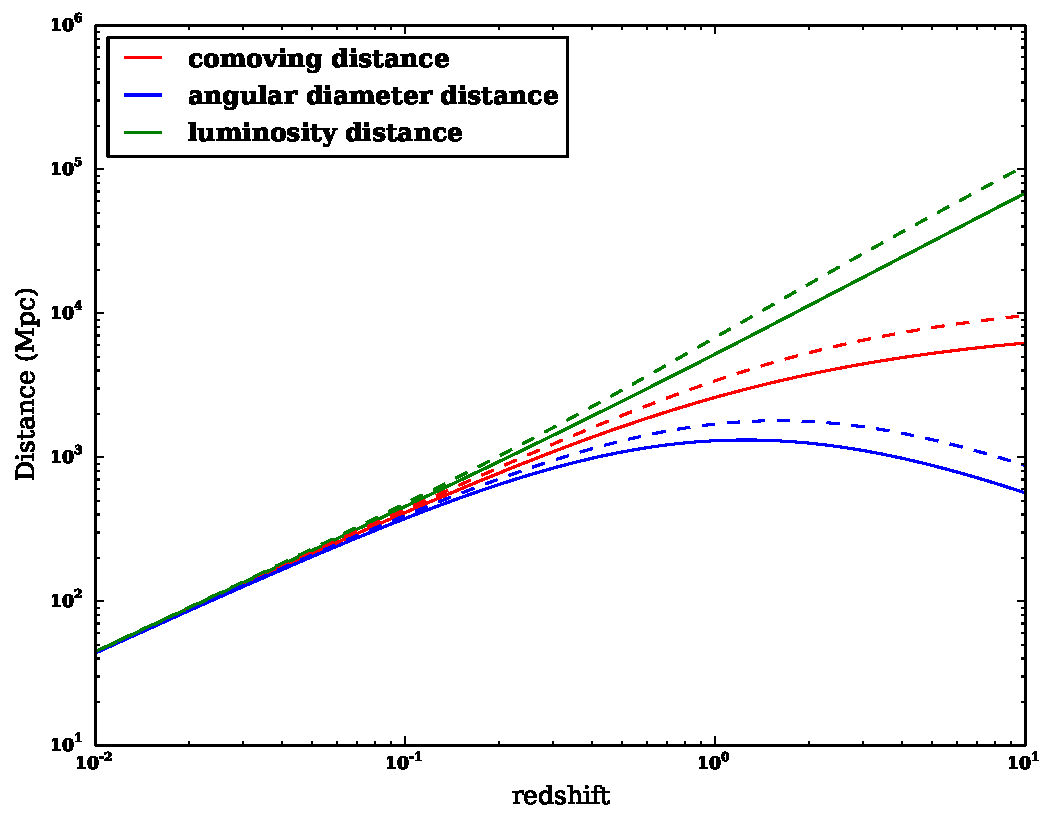
\includegraphics[width = \columnwidth]{figs/dist_redshift.pdf}
 \caption{Cosmological distances as a function of redshift - solid lines represent matter dominated universe and dashed lines represent \citet{planck18-6} cosmology. Measuring distance as a function of redshift provides valuable information on the constituent of the Universe. }
\label{fig:dist}
 \end{figure} 
 Fig. ~\ref{fig:dist} shows cosmological distances as a function of redshift; dashed lines represent the $Planck$ \citep{planck18-6} cosmology and solid lines represent matter only universe. 
 %Its worth here to note that the cosmological distances depend on the underlying cosmology. 
 %In fact the luminosity distances of supernovae were the first observational evidence of dark energy \pending{cite supernovae paper}.
  
 \section{Friedmann Equations}
The mathematical formalism of the universe so far based on the assumption of isotropy and homogeneity in an expanding universe which led us to the FLRW metric.
General theory of relativity relates the dynamics of the background universe to the matter and energy content in the universe via the Einstein Field Equations
\begin{equation}
 R_{\mu \nu} - \frac{1}{2} g_{\mu \nu} R = 8 \pi GT_{\mu \nu}.
\end{equation}
The L.H.S corresponds to the geometry of the universe, while the R.H.S represents the matter and energy content in the universe.
In the above equation $R_{\mu \nu}$ is the Ricci tensor which depends on the metric and its derivatives, R is the Ricci scalar and $g_{\mu \nu}$ is the metric.  The stress energy tensor, $T_{\mu \nu}$, is given by:
\begin{equation}
T^{\mu}_{\nu} = (\rho + P) u^{\mu} u _{\nu } - P \delta^{\mu}_{\nu}
\end{equation}
where $\rho(t)$ and P(t) are the energy density and pressure in the rest frame of the fluid and $u^{\mu}$ is the relative four velocity of the fluid.
Solving the time-time component of the Einstein field equation yields an equation for the evolution of the scale factor,
\begin{equation}
 H^2 = \left ({\dot a \over a} \right )^2 = \frac{8 \pi G}{3} \rho - \frac{k}{a^{2	}}
\label{Fred2}
\end{equation}
while all three spatial components reduce to 
\begin{equation}
\frac{\ddot{a}}{a} = -\frac{4 \pi G} {3} (\rho + 3P )
\label{Fred1}
\end{equation}
where $\rho$ = $\Sigma_{i} \rho_{i}$ and $P$ = $\Sigma_{i} P_{i}$ are the sum of energy density and pressure of all the components in the universe respectively.
 Equations ~\ref{Fred1} and ~\ref{Fred2} are the Friedmann equations governing the evolution of the background universe. \\\\  The average mass density of the Universe required to just halt the expansion of the Universe, it is given by, %For flat universe $k$  =0, it is given by
%  d In a flat universe ($k$ = 0) the kinetic energy of the universe is just enough to over the gravitational pull of the matter; the energy density which satifies this condition is called the critical density
 \begin{equation}
 \rho_{crit}  = \frac{3 H^{2}}{8\pi G}
 \end{equation}
Note that the value of critical density depends on Hubble's constant which is time dependent. The present value of critical density is approximately $10^{-26} kg/ m^{3}$. While this is equivalent to 6 hydrogen atoms per cubic meter, the best achievable terrestrial vacuum is $10^{9}$ atoms per cubic meter. The critical density can be used to define dimensionless density parameters as $\Omega_{i} = \rho_{i}/\rho_{crit}$. Assuming all the components in the universe are perfect isotropic fluids, we can write down the stress energy tensor as
\begin{equation}
T^{\mu}_{\nu} = 
\begin{pmatrix}
-\rho & 0 & 0 & 0 \\
0 & P & 0 & 0 \\
0 & 0 & P & 0 \\
0 & 0 & 0 & P 
\end{pmatrix}
\end{equation}
Using the energy-momentum conservation condition 
\begin{equation}
\dot \rho + 3\,H  (\rho + P) = 0
%\dot{\rho}  + H(3\rho + P)  = 0
\end{equation}
Note that the continuity equation will also hold for individual species as long as we neglect the energy exchange among different components. 
As mentioned earlier the cosmological fluids are expected to obey the equation of state: P = $w$ $\rho$. 
Plugging this in the above equation we can solve for density as function of scale factor
\begin{equation}
\rho(a) \propto \exp \left(-3 \int_1^a {da' \over a'} [1+w(a')] \right)
\end{equation}
For a time-independent equation of state parameter $w$ the above equation reduces to $\rho \propto a^{-3 (1+w)}$. 

The components of the Universe that we know about are:
\begin{itemize}
\item{\textbf{Non relativistic matter}}: For non-relativistic matter such as cold dark matter and baryons the energy density is equal to the rest mass energy. The pressure is much smaller than the energy-density ($P$ << $\rho$). In such cases $w =0$ and the density will scale as $\rho \propto a^{-3}$
\item{\textbf{Radiation and relativistic matter}}:  Pressure is related to the energy-density of relativistic matter as $P = 1/3 \rho$. This includes photons and neutrinos whose density scales with scale factor as $\rho \propto a^{-4}$
\item{\textbf{Dark Energy}}: It is a hypothetical form of energy which is responsible for late time cosmic acceleration. The equation of state parameter depends on the model of Dark Energy and in many of models the equation of state is time dependent. However the current data suggests the value equation of state parameter to be consistent with $w = -1$, with the \citet{planck18-6} indicating $w = -1.04 \pm 0.1$ . Substituting it in the above equation we get $\rho \propto a^{0}$ and hence the cosmic dilution doesn't affect the dark energy density. 
 \end{itemize}
 It is important here to note that the cosmic dilution has different effect on different components. While radiation component is subdominant in today's universe, it played a major role in the early universe. Fig. ~\ref{fig:scaling} shows the energy density of different components as a function of scale factor; as one expects at late times cosmological constant and matter are the dominant components, whereas at earlier times radiation plays a significant role in the evolution of background universe.
 \begin{figure}[ht]
 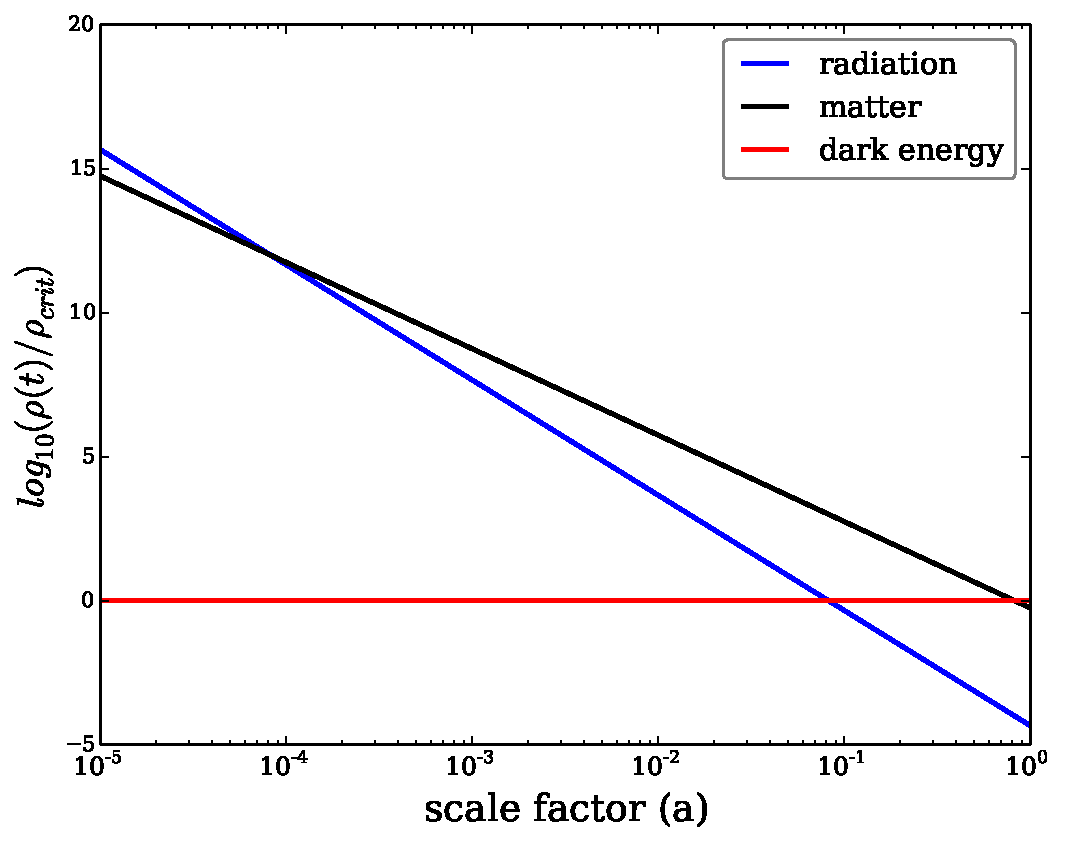
\includegraphics[width = \columnwidth]{figs/dummy.pdf}
 
 \caption{Scaling of various components as function of scale factor (a). While radiation is dominant component in the early universe, dark energy is dominant at present.}
 \label{fig:scaling}
 \end{figure}
With the density scaling relations in hand and substituting a = 1/(1+z), we can rewrite Eqn. ~\ref{Fred2} for a flat universe as 
\begin{equation}
H^{2}(z) = H^{2}_{0} (\Omega_{ro}(1+z)^{4} + \Omega_{mo}(1+z)^{3} + \Omega_{\Lambda}) 
\end{equation} 
where $\Omega_{ro}$,$\Omega_{mo}$ and $\Omega_{\Lambda}$ are the density parameters of radiation, matter and dark energy respectively. 
\iffalse{
 \section{Cosmic Inventory}
The above theoretical framework provides the evolution of different components as a function of scale factor. Now we look at the observational constraints obtained on these parameters. CMB temperature is measured precisely by the FIRAS instrument \cite{mather94} on COBE satellite \cite{fixsen96b}, $T = 2.725$ K $\pm$ 0.002K. %While neutrinos also contribute to radiation density, cosmic neutrinos have not been observed yet. 
For bosons such as photons the energy density as a function of temperature is given by 
\begin{equation}
\rho_{\gamma} = \frac{\pi^{2}}{15} T^{4}
\end{equation} 
which corresponds to 
\begin{equation}
\Omega_{\gamma} = \frac{\rho_{\gamma}}{\rho_{crit}} = 5.04 *10^{-5}
\end{equation}

Unlike photons the energy density of baryons cannot be obtained by measuring its temperature, it needs to be measured directly. 
There are two main independent ways to measure the baryon density: 
\begin{itemize}
\item Cosmic Microwave Background (CMB): by measuring the amplitude of the first and second peaks of CMB power spectrum
\item  Big Bang Nucleosynthesis (BBN): by measuring the primordial deuterium abundance.
\end{itemize}
From CMB power spectrum analysis we have $\Omega_{b} h^{2}$ = $0.0224 \pm 0.0001$  \cite{planck16-8} and that from BBN is $0.0226 \pm 0.00034$ \cite{cooke16}. Both of these measurements agree with each other remarkably well within error limits.


Dark matter forms 85\% of total matter content in the universe. Unlike baryons, dark matter doesn't interact with the radiation. 
As dark matter interacts only gravitationally, by measuring the gravitational field in a given system we can infer the total mass content. 
One of the ways to measure the total matter (dark matter + baryon) is by using galaxy cluster gas mass fraction. 
Galaxy clusters (detailed review is in next chapter) are so large that the ratio of gas mass to that of total cluster mass is expected to reflect the ratio baryon to the total mass in the universe\cite{white93a,grego01}. Constraints on dark matter density as measured by $Planck$ is $\Omega_{dm} h^{2} =  0.120 \pm 0.001$ \cite{planck16-8}.

As per current cosmological observations the major contribution for the energy density content in the universe is from dark energy. There are several observational probes to constrain this mysterious component which is responsible for the late time acceleration of the universe.  The first direct observational evidence is from type Ia supernovae. Supernovae have constant intrinsic luminosity and are known as standard candles. 
Cosmologists measured the luminosity distance (~\ref{eq:luminosity_dist}) of type Ia supernovaes as function of redshift to constrain $\Omega_{\Lambda}$  $\approx$ 0.7\citep{knop03}.
}\fi

\section{Cosmic Microwave Background}
Cosmic Microwave Background (CMB) was theoretically predicted by George Gamov in 1940s as an observational relic of Hot Big Bang model \citep{article46}. 
It was observed accidentally by Arno Penzias and Robert Wilson in 1964 at the Bell Laboratories for which there were awarded Nobel prize in physics in 1978 \citep{penzias65}. Almost three decades after its discovery, Cosmic Background Explorer (COBE) detected anisotropies in CMB at a tiny level of 10 in a million. Far-Infrared Absolute Spectrophotometer (FIRAS), an instrument mounted on COBE measured the black body spectrum of CMB \citep{mather94}. %temperature of CMB to be  $\sim$ 2.7K. 
Since then a number of experiments have been designed to measure the anisotropies in the CMB.

High density and temperature of the early universe ensured that all the components interacted with each other multiple times remaining in thermal equilibrium. 
Photons ($\gamma$), protons (p) and electrons (e) were tightly coupled into a state called photon-baryon plasma; proton and electrons interacted with each other through Coulomb scattering and photon interacted with electrons through Thompson scattering:
\begin{eqnarray}
\cee{p + e^{-} <=> H + \gamma}
\label{Coulomb}\\
\cee{\gamma + e^{-} <=> e^{-} + \gamma}
\end{eqnarray} 
As the universe expands the mean energy density dilutes and the temperature decreases. When the temperature falls below the ionization energy of hydrogen, E < 13.6 eV the reaction in Eq.~\ref{Coulomb} thermodynamically favours to  $\cee{p + e^{-} -> H + \gamma}$ \footnote{To be precise, recombination occurs at slightly lower temperature (~1MeV) due to the large over abundance of photons with respect to baryons}. This results in the creation of neutral hydrogen atoms and the electron density decreases, which results in the decoupling of photons from the baryons. This epoch is called the epoch of recombination; observations determine that it happened at redshift of  $z$ = $1089.90 \pm 0.23$ \citep{planck18-6}. 

As a first light from the early universe, the CMB provides a wealth of cosmological information. The theory of inflation is able to describe the homogeneity measured in the CMB. The inhomogeneties are only of order of 10 in a million which can be directly measured from the observed anisotropies in CMB. %Over the evolution of the universe slightly over dense regions of the early universe collapsed gravitationally to form the large scale structures that we see today. Analysing these structures involve complicated non-linear physics, however, CMB can be analysed linearly. In addition to that, $z \sim 1100$ provides long lever arm on the geometry of the universe.

\begin{figure}[ht]
\includegraphics[width = \columnwidth]{figs/CMB_map.pdf}
 \label{cmb map}
 \caption{CMB anisotropies as observed by $Planck$ satellite. Credits: ESA/$Planck$ collaboration}
\end{figure}
\iffalse{
\section{Boltzmann equations}
\label{eqns}
In the early universe photons, baryons, and dark matter are tightly coupled to each other in a complicated way. 
The systematic way to understand these couplings is by using Boltzmann equations. 
Boltzmann equations are easier to solve in Fourier space, as different Fourier modes evolve independently in linear approximation. 
This section closely follows \pending{Scott and Dodelson}, here I summarize the Boltzmann equations for cold dark matter, photons, and baryons which were the dominant component of the universe at recombination.


The evolution of photon distribution is coupled to electrons and metric. Photon Boltzmann equation in the Fourier space is given by:
\begin{equation}
\dot{\tilde{T}} + i k(\hat{k}. \hat{p}) \tilde{T} + \dot{\tilde{\Phi}} + i k (\hat{k}.\hat{p}) \tilde{\Psi} = \dot{\tau}[\tilde{T_{0}} - \tilde{T} + (\hat{k}.\hat{p})\tilde{v_{b}}]
\end{equation}
where T represents the photon temperature, $\hat{p}$ is the photon direction, $v_{b}$ is the electron velocity, and $\tau$ is the optical depth.
Variables with $\tilde{}$ denotes Fourier transform, ones with $\dot{}$ denotes derivative with respect to conformal time $\eta$.
$\dot{\tilde{\phi}}$ and $\dot{\tilde{\psi}}$ represent the conformal time derivative of the metric. 

Cold dark matter (CDM) evolution is the simplest among all as it has only two free parameters velocity and density. 
CDM Boltzmann equation is given by:
\begin{eqnarray}
\dot{\tilde{\delta}} + ik\tilde{v} + 3 \dot{\tilde{\Phi}} = 0\\
\dot{\tilde{v}} + \frac{\dot{a}}{a} \tilde{v} + ik \tilde{\Psi} = 0
\end{eqnarray}
where $v$ is the dark matter velocity, a is the scale factor, and $\delta$ is the fractional dark matter over density 
\begin{equation}
\delta = \frac{\delta \rho}{\rho} 
\end{equation}
$\rho$ is the dark matter density.

Proton and electrons are tightly coupled to each other by Coulomb forces. In addition to that the electrons also interact with photons through Thompson scattering. 
Both protons and electrons are analysed together as baryons, the Boltzmann equation for baryons is given by
\begin{eqnarray}
\dot{\tilde{\delta_{b}}} + ik\tilde{v_{b}} + 3 \dot{\tilde{\Phi}} = 0 \\
\dot{\tilde{v_{b}}} + \frac{\dot{a}}{a} \tilde{v_{b}} + i k \tilde{\Psi} = \dot{\tau}\frac{4\rho_{\gamma}}{3\rho_{b}} [3i\tilde{T_{1}} + \tilde{v_{b}}]
\end{eqnarray}
where $\rho_{\gamma}$ and $\rho_{b}$ are the photon and baryon density respectively; $T_{1}$ is the first moment of photon temperature. 

All the above Boltzmann equations can be solved numerically to a great precision for a given cosmological model by using publically available codes such as CAMB \citep{lewis00} and CMBFAST \citep{seljak96}.
\begin{figure}[ht]
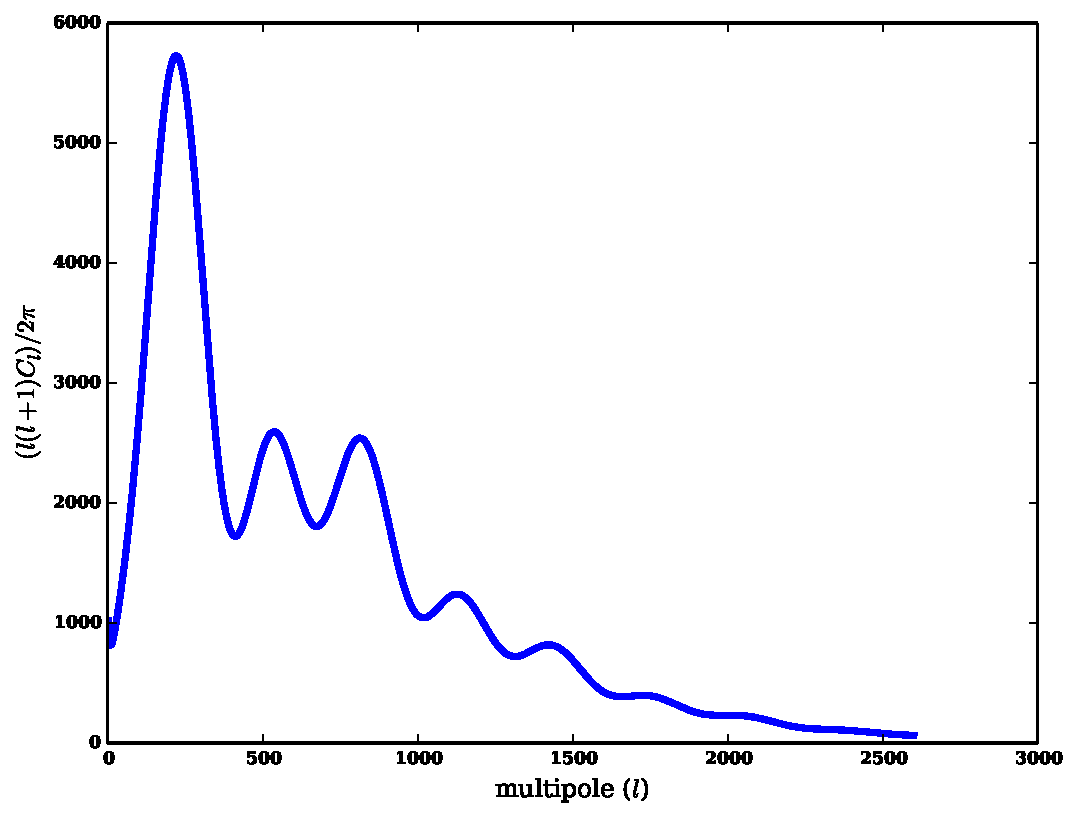
\includegraphics[width = \columnwidth]{figs/cmb_ps.pdf}
\caption{Angular power spectrum of CMB primary temperature anisotropies for $Planck$ cosmology \citep{planck18-6}.}
\label{fig:cmb_ps}
\end{figure}
}\fi
\section{Temperature primary anisotropies}
 The measured CMB temperature in a given direction $\hat{n}$ can be written as:
\begin{equation}
T = T_{0}\left(1+ \vec{\beta}.\hat{n} + \frac{T(\hat{n})}{T_{0}}\right)
\end{equation}
where $T_{0}$ is the average CMB temperature, $\vec{\beta} $ is the dipole term due to the relative velocity of Earth with respect to Hubble flow. Here $\beta$ is equal to $\frac{\vec{v}}{c}$ where $\vec{v}$ is the Earth's relative velocity. 
The last term in the equation represents the anisotropies in the CMB which here after we denote by $\Phi(\hat{n})  = \frac{T(\hat{n})}{T_{0}}$. 
Note that in the above equation we have ignored foregrounds, systematics, and experimental noise. %The oder of the anisotropies ($\phi$) is two orders of magnitude smaller than effect due to doppler boost. 

Given the stochastic nature of fluctuations in CMB, we cannot predict the value of temperature at a given location. However, we can predict the statistical properties. 
As an function on the surface of sphere, CMB fluctuations can be decomposed in terms of spherical harmonics as follows:
\begin{eqnarray}
\Phi(\hat{n}) = \Sigma_{l} \Sigma_{m} a^{T}_{lm} Y_{lm} (\hat{n}) \\
a^{T}_{lm} = \int d\Omega \Phi(\hat{n}) Y_{lm} (\hat{n})
\end{eqnarray}
where $Y_{lm}$ are the spherical harmonic basis, %used to define function on a sphere
$a^{T}_{lm}$ are the harmonic coefficients. 
It is important to note here that angular scale $\theta$ is related to multipole $l$ as $\theta \sim 1/l$. 

The randomness of the fluctuations wont let us predict the value of the harmonic coefficient $a^{T}_{lm}$. However, theories do predict the distribution from which the $a^{T}_{lm}$ are picked. In the inflationary paradigm CMB fluctuations are realisations of a  Gaussian random field, meaning that the harmonic coefficients are drawn from random Gaussian distribution\footnote{It must be noted that most of the inflationary models predict a small amount of non-Gaussianity.}. The harmonic coefficients satisfy 
\begin{eqnarray}
\langle a^{T}_{lm} \rangle = 0,\\
\langle a^{T}_{lm} a^{T*}_{l'am'}\rangle = \delta_{l l'}\delta_{m m'} C^{TT}_{l},\\
a^{T}_{l-m} = (-1)^{m}a^{T*}_{lm}
\end{eqnarray}
where $\langle \rangle$ denotes the ensemble average over many realisations, $C^{TT}_{l}$ is the angular power spectrum of CMB. 

Our universe is only one of many realisations of the Gaussian random field, so we face fundamental limits on the knowledge available. This is known as cosmic variance.
 However, we can still calculate the angular power spectrum.
The idea is to replace the ensemble average with the spatial sample average i.e averaging over $2l +1$ samples. 
\begin{equation}
\hat{C}^{X}_{l} = \frac{1}{2l +1}\Sigma_{m} |a^{X}_{lm}|^{2}
\end{equation}
where X $\epsilon$ (T,E,B) - T is the temperature mode and E, B are the polarisation modes .
This measured power spectrum is fitted to the theoretical power spectrum to extract cosmological information. For historical reasons the CMB power spectrum is conventially parameterized as 
 \begin{equation}
 D_{l} = \frac{l(l+1)}{2\pi} C_{l}.
 \end{equation}
 
 The theoretical CMB power spectrum for standard $\Lambda CDM$ cosmology as obtained from CMBFAST \citep{seljak96} is show in Fig. ~\ref{cmb_ps}. A wealth of cosmological information can be obtained from CMB power spectrum and below I discuss three main features (it closely follows \citet{douglas2010}):
 
\begin{figure}[ht]
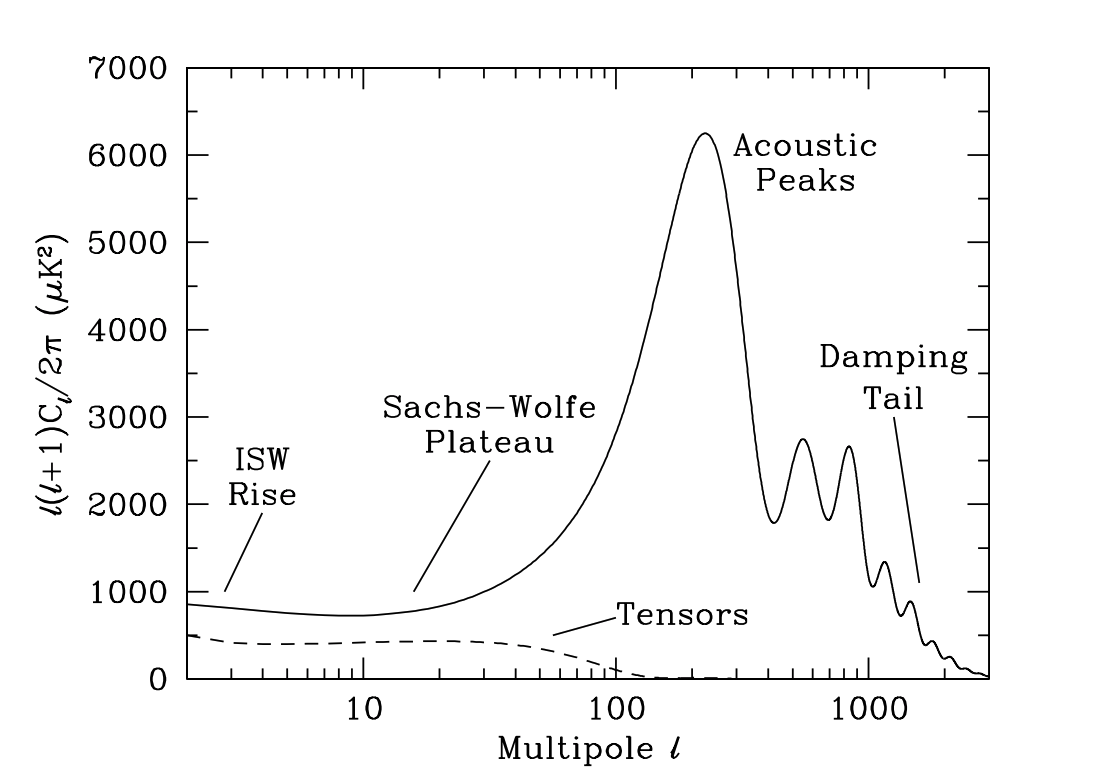
\includegraphics[width = \columnwidth]{figs/cmb_ps_sd.png}
\caption{The theoretical CMB power spectrum as obtained from CMBFAST \citep{seljak96}}
\label{cmb_ps}
\end{figure}

 \textbf{Sachs-Wolfe Plateau:}
 
 The horizon scale at last scattering surface corresponds to multipole $l \approx 100$. At these scales the anisotropies have not evolved significantly and hence faithfully trace initial condition. $\delta T/ T \approx  1/3 \delta \phi c^{2}$, where $\delta \phi $ is the perturbation to the gravitational potential evaluated on the last scattering surface (LSS) \citep{sachs67}.
 
 \textbf{Acoustic oscillations:}
 
On sub-degree scales, corresponding to multipole range $ 100 \le l \le 1000 $, the rich structure in the power spectrum is due to gravity-driven acoustic oscillations occurring before the atoms in the Universe became neutral. Perturbations inside the horizon at last scattering have been able to evolve causally and produce anisotropy at the last scattering epoch, which reflects this evolution. The frozen-in phases of these sound waves imprint a dependence on the cosmological parameters, which gives CMB anisotropies their great constraining power. Location and height of acoustic peaks are sensitive to various cosmological parameters especially curvature of the Universe, dark energy, amount of baryons, optical depth, and dark matter \citep{hinshaw13,planck18-6}. 
 
\textbf{Damping tail:}

The recombination process is not instantaneous, giving a thickness
to the last scattering surface. This leads to a damping of the anisotropies at the highest $l$s, corresponding to scales smaller than that subtended by this thickness. One can also think of the photon-baryon fluid as having imperfect coupling, so that there is diffusion between the two components, and hence the amplitudes of the oscillations decrease with time. These effects lead to a damping of the $C_{l}$s, sometimes called Silk damping \citep{silk68}, which cuts off the anisotropies at multipoles above about 2000 \citep{keisler11,story13,das11b,reichardt09a}.   

The CMB interacts with the intervening medium (between last scattering surface and us) and this imprints secondary anisotropies. Secondary anisotropies also provide wealth of cosmological information especially on structure formation and epoch of reionisation \citep{lueker10,shirokoff11,flower10,das11}. 

\section{CMB polarisation}
\begin{figure}[ht]
 \includegraphics[width = \columnwidth]{figs/quadrupole.pdf}
\caption{The above figure depicts important scenarios as experienced by an electron at the time recombination; it is adopted from the works of \cite{hu97d} and \cite{dodelson_book}. }
\label{quadrupole}
\end{figure}

The CMB is partially polarised linearly at the 10\% level due to the Thompson scattering of photons by electrons at the surface of last scattering. 
Only quadrupole anisotropy is responsible for CMB polarisation as shown in Fig. ~\ref{quadrupole}. 
 The Fig. ~\ref{quadrupole} represents important scenarios experienced by electron at the time of recombination. Red and blue represent relatively hot and cold photons respectively; green represents the average temperature. 
 Image on the top left represents the isotropic scenario which results in no net anisotropy.
 On the top right is that of dipole anisotropy which also results in no net polarisation. 
 Only the quadrupole anisotropy which is shown in the bottom panel results in net linear polarisation. 


The polarisation pattern on the CMB sky can be decomposed into curl-free E-modes, and
divergence-free B-modes. This is similar to Maxwell?s equation where the curl of the electrostatic
field, and the divergence of the magnetic field are zero. The reason the polarisation
patterns are called E, B modes is because of this similarity to electromagnetism.
\begin{eqnarray}
\vec{\nabla} \times \vec{E} = 0\\
\vec{\nabla} . \vec{B} = 0
\end{eqnarray}

The most important reason for this decomposition is that the scalar perturbations only
generate E-modes but does not generate B-modes, and the tensor perturbations generate both
E, and B-modes in equal amounts.
 %Before recombination photons and electrons were tightly coupled resulting no net local anisotropy. 
%However, during the period of recombination there is slight anisotropy between photons and free electrons. 
Though CMB polarisation signal is weak compared to its temperature counterpart, it provides invaluable information on inflation and on late time evolution of universe through its lensing effects and the imprint of primordial gravitational waves on tensor B-modes
In addition to that, foregrounds are only partially polarised.
The CMB polarisation was first detected observationally by Degree Angular Scale Interferometer (DASI) in 2002 \citep{kovac02}.
Since then measurement of CMB polarisation has been done by SPT \citep{henning18,sayre19,keisler15}, ACT \citep{louis16,naess14}, $Planck$ \citep{planck19},  BICEP2/Keck \citep{bicep18,bicep15}, and POLARBEAR \citep{polarbear2014b,wald2019}. %numerous experiments which have measured CMB polarisation \citep{sayre19,henning18,bicep18,keisler15,polarbear2014b}.

 
 
 \section{Other cosmological probes}
 
 In addition to CMB there are other cosmological probes which provide invaluable and complementary insight into the standard model of cosmology. Below I provide a very brief discussion of other cosmological probes.
 
 
 \textbf{Supernovae:}
 
Type Ia supernovaes are excellent standard candles for measuring the expansion history of the Universe and provided the first direct evidence of dark energy \citep{riess98,perlmutter99a,perlmutter99b}. Theoretical models suggest that these ``standard candles'' arise because of thermonuclear explosion of a carbon-oxygen white dwarf that has grown to the Chandrashekar mass.
%Type Ia supernovae are thought to be result of explosion of white dwarf in a binary system. 
These events have well defined Hubble diagram whose intercept provides a robust measurement of  Hubble constant. The value of hubble constant measured using Type Ia supernovae data from Dark Energy Survey is $H_{O} = 67.8 \pm 1.3 \; \si{\km\per\s}\si{\per\mega\parsec}$ \citep{macaulay2018}. %will and by measuring their brightness we can measure how far supernovae are  and hence the expansion of the Universe. 
 


 \textbf{Baryon Acoustic Oscillations:}
  
While supernovae acts as ``standard candles'', Baryon Acoustic Oscillations (BAO) acts as standard rulers in cosmology. 
 They are the frozen relics left over from the pre-decoupling universe. As such, probing the BAO scales at different times provides valuable cosmological information. 
 The best measurement BAO scale comes from CMB anisotropy measurements at redshift $z \approx 1100$ \citep{planck18-6}. BAO are also present in
the distribution of matter, and there are measurements at low redshifts using the clustering of galaxies \citep{beutler11,ross15,alam16}.
BAO data can only constrain a combination of the size of the sound horizon and the expansion rate of the Universe ($H_{o}$). Usually CMB anisotropy measurements are used to break this degeneracy. Using the Big Bang Nucleosynthesis prior and latest data from eBOSS DR14, \citet{andrei14} measured $H_{O} = 67.6 \pm 1.1 \si{\km\per\s}\si{\per\mega\parsec}$. 
 
 
 %\textbf{Redshift Space Distortions (RSD}
  
 
